% !TEX root = ../IS.tex
\chapter{Description of Software}
\section{AI Model}
To begin building an AI model, I first created a simulation of the game. The simulation had two players, each with 25 health points (HP). Both players had two possible actions per turn, which were randomly selected: attack the other player, reducing their opponents HP by 5 points, or heal themselves, increasing their HP by 4 points. Each action had a 50\% chance of occuring. The game ran until one player's HP was reduced to 0. The total number of turns and the sequence of actions were recorded into a CSV file. After running 4500 simulations, the data was imported into Matlab. A subset of the games were used as a training set for a decision tree, which would predict which player would win the game.\\

\begin{figure}[H]
  \centering
  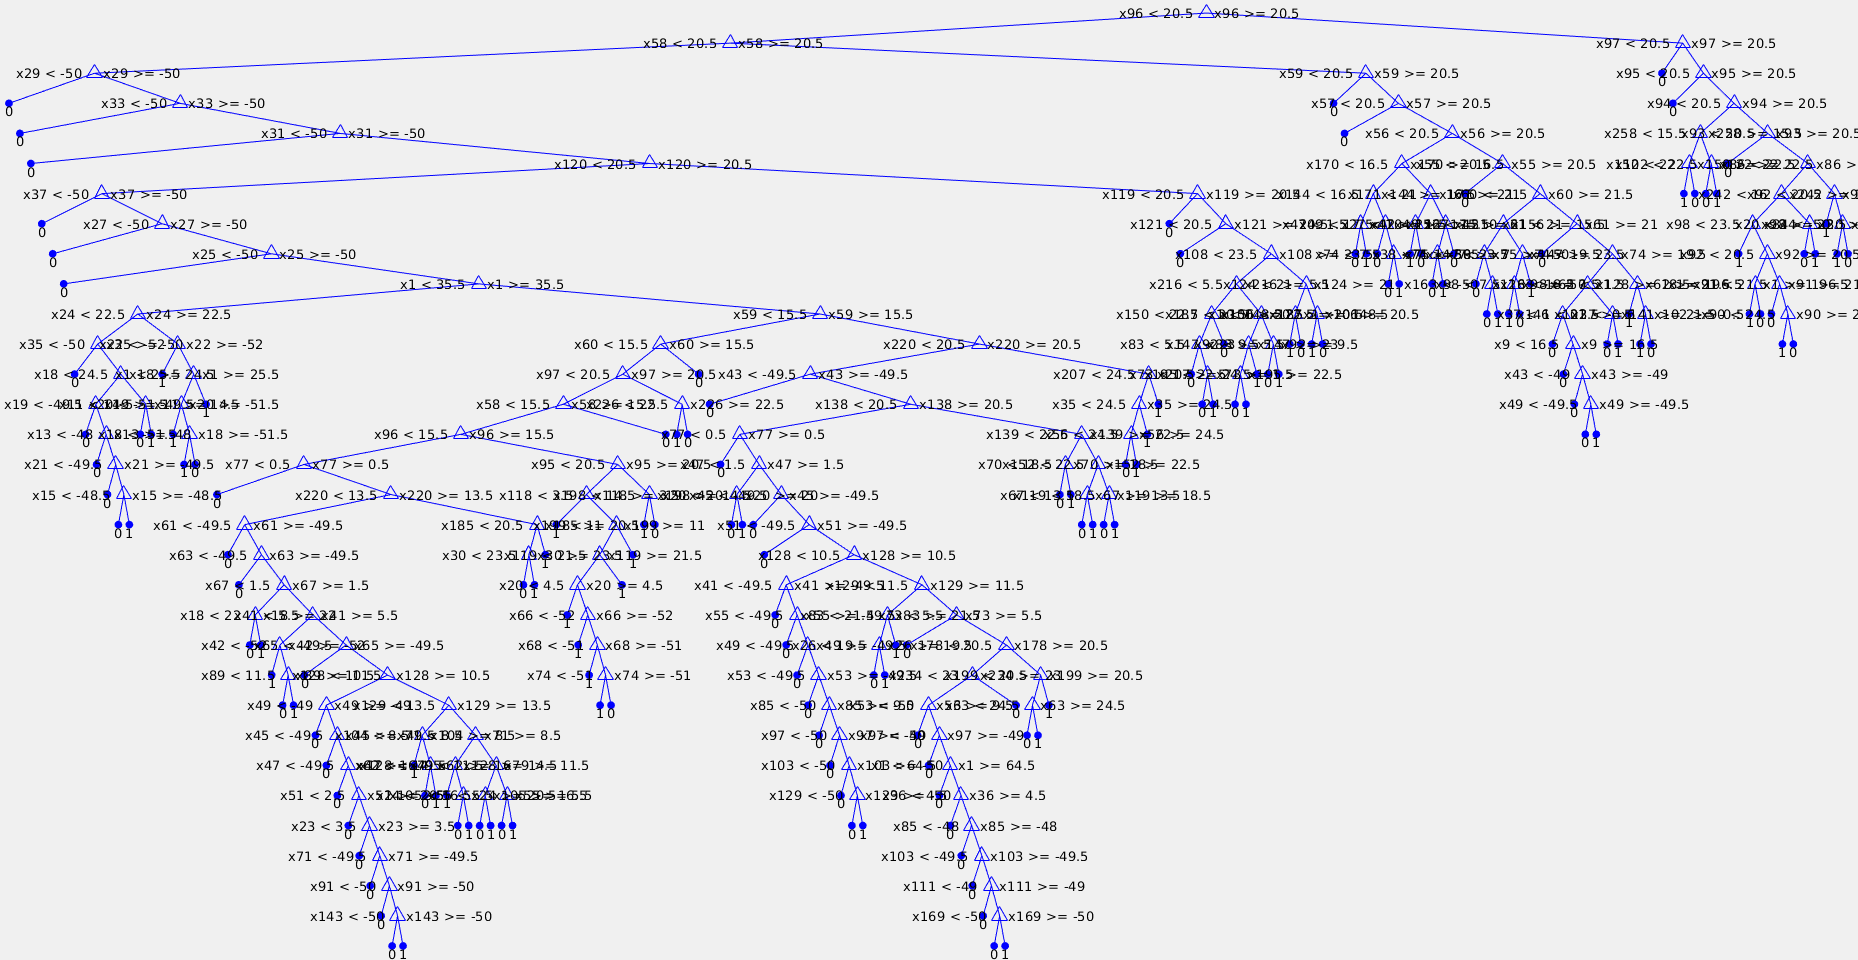
\includegraphics[width=12cm]{figures/firstDecisionTree.png}
  \caption{The decision tree generated from 4000 simulations of the game. This tree predicts 0 when player 1 wins and 1 when player 2 wins.}
  \label{fig:decisionTree1}
\end{figure}

However, this method was inconclusive, for a number of reasons. Firstly, the decision tree included a large number of branches, as seen in Figure \ref{fig:decisionTree1}. Secondly, the actual criteria being evaluated at each branch of the tree is different for each game. Aside from the first column, which contained the total number of turns in the game, and the second column, which contained the starting HP of player 1, the values in any particular column will differ from game to game. For instance, the root node used the value in column 96 as its classifier. In one game, column 96 may contain a HP value for player 2. In another, longer game, that column may contain a HP value for player 1. Thirdly, the individual games 
\section{Game Engine}
\subsection{The Pygame Library}
The Pygame library provides a number of Python functions that are useful in creating a two-dimensional video game. The library was originally created in 2001 to combine Python with SDL (Simple DirectMedia Layer), a library of multimedia controls written for C \cite{shinners}. Pygame can utilize a variety of different graphics libraries, including OpenGL, DirectX, the Linux frame buffer, and an ASCII art backend \cite{shinners}. The pygame library is supported by a dearth of operating systems, and the core functions of pygame use highly optimized C or assembly code.\\

At the top level, Pygame controls the initialization and exiting of its various modules, particularly the pygame.display module which renders the game. Pygame features two functions to update a display window, pygame.display.flip() and pygame.display.update(). display.flip() works as a standard buffer swap, reloading the entire display with the new information in a frame buffer. display.update() is an optimized version of flip(), which can take as an argument a rectangle or sequence of rectangles. These rectangles correspond to the areas of the display which need to be updated. For instance, passing the coordinates of a rectangle over a game's scoreboard will only update the scoreboard.\\

The two main objects in Pygame are the Surface object and the sprite object. Surfaces can be changed with Pygame to alter their color palette, bitmasks, and alpha value. Surfaces are mostly used to load image files and to create backgrounds for the game. Sprites, on the other hand, are used for the actual in-game objects, such as enemies, player characters, and projectiles. Sprites can be stored in a Group object, which can be used to separate sprites by different purposes. Each sprite draws its image to a Surface, provided that it has a Surface.image and Surface.rect attribute.\\

Once a sprite or surface has been created with an image, Pygame can also perform graphical transformations on that image. The pygame.transform module has functions to flip, rotate, and scale an image. Another Pygame feature is the ability to do collision detection on sprites and rectangles.\\

For the actual gameplay of a Pygame program, there are also modules for joystick, mouse, and keyboard controls. A sound mixer module allows audio tracks to be played in the game, and the pygame.time module controls the framerate of the game.